\section{Objetivos}

\subsection{Objetivo general:}

Desarrollar un prototipo funcional para la deteccion y clasificacion local de manchas solares, integrando técnicas de visión por computadora, inteligencia artificial y análisis predictivo de actividad solar para observatorios locales.

\subsection{Objetivos específicos:}

\begin{itemize}
    \item Analizar registros históricos de manchas solares a partir de imágenes heliográficas y datos astronómicos.
    \item Diseñar un flujo de adquisición y preprocesamiento de imágenes para vincular imágenes de manchas solares con reportes internacionales.
    \item Desarrollar un detector basado en arquitecturas de Deep Learning modernas para localizar grupos solares y un clasificador jerárquico de inferencia de caracteres Zurich-–McIntosh preservando la dependencias semánticas.
    \item Implementar un módulo predictivo que aporte contexto operacional sobre la evolución temporal del índice de manchas solares y la distribución latitudinal de la actividad a partir de registros históricos.
    \item Integrar el sistema en una arquitectura híbrida con plataforma web y procesamiento inferencial local.
    \item Validar el funcionamiento integral del sistema mediante métricas de detección, clasificación, coherencia predictiva y consistencia física sobre datos históricos y escenarios de uso real.
\end{itemize}


\begin{figure*}[t]
    \centering
    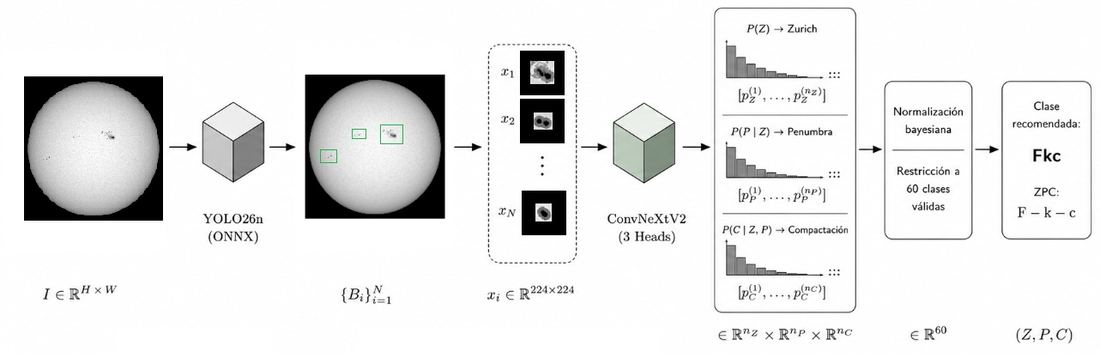
\includegraphics[width=0.98\linewidth]{figures/sys/img_pipe.jpg}
    \caption{Propuesta modular de detección y clasificación de manchas solares \textbf{Fuente:} Elaboración propia.}
    \label{fig:resumen-flujo-general}
\end{figure*}